\section{Wavelet Adaptive Mesh Refinement}
\label{sec:wamr}

Dendro employs wavelet adaptive mesh refinement (WAMR) to construct a sparse representation of the evolved fields while maintaining resolution in regions where the solution contains significant spatial structure. The basic idea is to represent the computational domain using a hierarchy of nested dyadic grids. In one spatial dimension, these grids may be written as
\begin{equation}
    V_j
    =
    \left\{
        x^{j,k}
        =
        2^{-j} k\,\Delta x
    \right\},
\end{equation}
where $j$ denotes the refinement level, $k$ indexes the points on that level, and $\Delta x$ is the spacing on the coarsest grid. If the physical domain has length $L$ and the base grid $V_0$ contains $N+1$ points, then
\begin{equation}
    \Delta x = \frac{L}{N}.
\end{equation}
The grids are nested, so points present on a coarse level also appear on all finer levels. In particular, points with even index on level $j+1$ coincide with points on level $j$,
\begin{equation}
    x^{j+1,2k} = x^{j,k}.
\end{equation}
The multidimensional AMR hierarchy used in the simulations is built from the same dyadic refinement idea.

Figure~\ref{fig:wamr grid hierarchy} illustrates this nested structure in one dimension. The black points denote grid points inherited from coarser levels, while the red points denote the additional points introduced at each refinement level. These additional points form the detail spaces $W_j$, which contain the information added when passing from level $j-1$ to level $j$.

\begin{figure}[t]
\centering
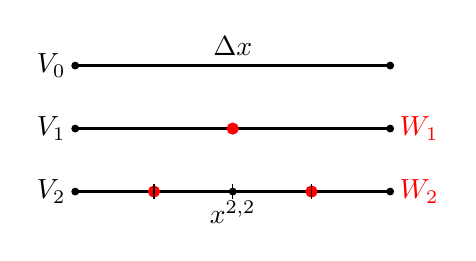
\begin{tikzpicture}[scale=1]
    % V0 line
    \draw[thick] (0,0) -- (4,0);
    \node[left] at (0,0) {$V_0$};
    \node[above] at (2,0) {$\Delta x$};

    % Endpoints for V0
    \filldraw (0,0) circle (1.2pt);
    \filldraw (4,0) circle (1.2pt);

    % V1 line
    \draw[thick] (0,-0.8) -- (4,-0.8);
    \node[left] at (0,-0.8) {$V_1$};
    \node[right, red] at (4,-0.8) {$W_1$};
    \filldraw (0,-0.8) circle (1.2pt);
    \filldraw[red] (2,-0.8) circle (2pt);
    \filldraw (4,-0.8) circle (1.2pt);

    % V2 line
    \draw[thick] (0,-1.6) -- (4,-1.6);
    \node[left] at (0,-1.6) {$V_2$};
    \node[right, red] at (4,-1.6) {$W_2$};
    \filldraw (0,-1.6) circle (1.2pt);
    \filldraw[red] (1,-1.6) circle (2pt);
    \filldraw (2,-1.6) circle (1.2pt);
    \filldraw[red] (3,-1.6) circle (2pt);
    \filldraw (4,-1.6) circle (1.2pt);
    \node[below] at (2,-1.6) {$x^{2,2}$};

    % Ticks
    \foreach \x in {1,2,3} {
        \draw (\x,-1.5) -- (\x,-1.7);
    }
\end{tikzpicture}
\caption{
Schematic illustration of the nested dyadic grids used in wavelet adaptive mesh refinement. Points present on coarser grids are retained on finer grids, while the red points indicate the additional degrees of freedom introduced at each refinement level. These additional points correspond to the detail spaces $W_j$.
}
\label{fig:wamr grid hierarchy}
\end{figure}

Let $u^{j,k}$ denote the value of a field $u$ at the grid point $x^{j,k}$. Since the grids are nested, values at points inherited from the previous level satisfy
\begin{equation}
    u^{j+1,2k}
    =
    u^{j,k}.
\end{equation}
The values at newly introduced points may be estimated by interpolation from the previous level,
\begin{equation}
    u^{j+1,2k+1}
    =
    \sum_m h^{j+1,2k+1}_{j,m}\,u^{j,m},
\end{equation}
where $h^{j+1,2k+1}_{j,m}$ are the interpolation weights. In practice only a small number of these coefficients are nonzero. For the fourth order interpolation used here, the interior interpolation stencil is
\begin{equation}
    u^{j+1,2k+1}
    =
    -\frac{1}{16}u^{j,k-1}
    +\frac{9}{16}u^{j,k}
    +\frac{9}{16}u^{j,k+1}
    -\frac{1}{16}u^{j,k+2}.
\end{equation}
Near physical boundaries the same interpolation idea is used, but the stencil is shifted so that it remains inside the domain, leading to modified one sided interpolation weights.

Equivalently, this interpolation can be described in terms of scaling functions. A basis function on level $j$ may be represented using basis functions on the finer level $j+1$ as
\begin{equation}
    \phi_{j,k}(x)
    =
    \sum_l c_l\,\phi_{j+1,l}(x),
\end{equation}
where the coefficients $c_l$ encode the interpolation stencil. For the fourth order stencil above, the corresponding nonzero two scale coefficients are
\begin{equation}
    c_l
    =
    \left\{
        \ldots,
        0,
        -\frac{1}{16},
        0,
        \frac{9}{16},
        1,
        \frac{9}{16},
        0,
        -\frac{1}{16},
        0,
        \ldots
    \right\}.
\end{equation}
Each basis function may be viewed as a scaled and translated copy of a single fundamental interpolating function,
\begin{equation}
    \phi_{j,k}(x)
    =
    \phi\!\left(\frac{2^j x}{\Delta x} - k\right).
\end{equation}

The nested nature of the grids introduces redundancy if basis functions are included for every point on every level. To avoid this, one introduces alternate grids $W_j$ for $j>0$, consisting only of the points that first appear at level $j$:
\begin{equation}
    W_j
    =
    \left\{
        x^{j,k} : x^{j,k}=2^{-j}k\Delta x,
        \quad k \ \mathrm{odd}
    \right\}.
\end{equation}
Thus the collection $\{V_0,W_1,W_2,\ldots\}$ represents each grid point exactly once. The corresponding index sets are
\begin{equation}
    S_0 = \{0,1,\ldots,N\},
    \qquad
    S_j = \{1,3,\ldots,2^jN-1\},
\end{equation}
where $S_0$ labels the base grid and $S_j$ labels the detail points on level $j$.

This nested basis construction allows the field to be represented by a coarse contribution together with corrections from the detail spaces. A field can be expanded as
\begin{equation}
    u(x)
    =
    \sum_{k \in S_0}
    u^{0,k}\,\phi_{0,k}(x)
    +
    \sum_{j=1}^{J}
    \sum_{k \in S_j}
    d^{j,k}\,\phi_{j,k}(x),
\end{equation}
where $u^{0,k}$ are the base level field values and $d^{j,k}$ are the wavelet coefficients. This is the interpolating wavelet representation of the field. The first term gives the coarse representation on the base grid, while the remaining terms give the corrections required at successively finer levels.

The wavelet coefficient at a detail point is computed by comparing the actual field value to the value predicted by interpolation from the previous refinement level,
\begin{equation}
    d^{j,k}
    =
    u^{j,k}
    -
    P\!\left(x^{j,k},j-1\right),
\end{equation}
where $P(x^{j,k},j-1)$ denotes the interpolated value obtained from level $j-1$. Thus, the coefficient $d^{j,k}$ measures the local interpolation error associated with omitting the point $x^{j,k}$. This transformation from point values to wavelet coefficients is the forward wavelet transformation. It can be inverted by reconstructing the field values from the base level values and the wavelet coefficients.

There are therefore two equivalent descriptions of the field on the multi level grid. The first is the point representation, given by the field values $\{u^{j,k}\}$. The second is the wavelet representation, given by the base values and wavelet coefficients,
\begin{equation}
    \{u^{0,k},d^{j,k}\}.
\end{equation}
The wavelet representation can be made sparse by discarding points whose wavelet coefficients are below a prescribed tolerance $\varepsilon$,
\begin{equation}
    |d^{j,k}| < \varepsilon .
\end{equation}
These discarded points are well approximated by interpolation from coarser levels. The retained points are called essential points, and all base level points are always retained. The field values on the essential points form the sparse point representation. For interpolating wavelets, thresholding the coefficients also provides an a priori control of the representation error, with constants determined by the interpolation basis.

In practice, refinement is controlled by the tolerance $\varepsilon$, and detail points are retained when, schematically,
\begin{equation}
    |d^{j,k}| > \varepsilon .
\end{equation}
This criterion provides an efficient adaptive representation: smooth regions of the solution are represented using relatively few points, while regions containing sharp gradients, wave propagation, or strong field structure are refined automatically.

In higher dimensions the construction is extended by taking tensor products of the one dimensional basis functions. In three spatial dimensions,
\begin{equation}
    \phi_{j,\mathbf{k}}(x,y,z)
    =
    \phi_{j,k_x}(x)
    \phi_{j,k_y}(y)
    \phi_{j,k_z}(z),
\end{equation}
where $\mathbf{k}=(k_x,k_y,k_z)$. Equivalently, interpolation can be performed directly in multiple dimensions. Depending on the location of the new point relative to the previous level, the interpolation stencil may involve $p$, $p^2$, or $p^3$ points, where $p$ is the one dimensional interpolation order. The wavelet coefficient is again computed as the difference between the actual field value and the value interpolated from the previous level.

The multidimensional wavelet expansion has the form
\begin{equation}
    u(x,y,z)
    =
    \sum_{\mathbf{k}}
    u^{0,\mathbf{k}}\,
    \phi_{0,\mathbf{k}}(x,y,z)
    +
    \sum_{j=1}^{J}
    \sum_{\mathbf{k}}
    d^{j,\mathbf{k}}\,
    \phi_{j,\mathbf{k}}(x,y,z).
\end{equation}
As in one dimension, sparse refinement is obtained by retaining only those points whose wavelet coefficients exceed the chosen tolerance. This produces an adaptive multi level grid that concentrates resolution where the evolved fields are not accurately represented by interpolation from coarser levels.

\section{Sobolev Informed Refinement}
\label{sec:sobolev amr}

In addition to the standard wavelet criterion, we also consider a Sobolev inspired modification of the refinement. The purpose of this modification is to make the refinement criterion sensitive not only to the local wavelet truncation estimate of a field, but also to local derivative content. This is useful in regions where the field itself may be relatively smooth in amplitude, while its gradients or curvature contain dynamically relevant structure.

For a given evolved variable $u$, the standard wavelet refinement indicator may be denoted by
\begin{equation}
    I_{\mathrm{W}}(u).
\end{equation}
This quantity represents the usual WAMR estimate based on the magnitude of the local wavelet coefficient. The Sobolev informed indicator augments this quantity by including contributions from first and second spatial derivatives. We use an indicator of the form
\begin{equation}
    I_{\mathrm{Sob}}(u)
    =
    \sqrt{
        I_{\mathrm{W}}(u)^2
        +
        w_1 I_{\nabla u}^2
        +
        w_2 I_{\nabla^2 u}^2
    },
    \label{eq:sobolev amr indicator}
\end{equation}
where $I_{\nabla u}$ is a local first derivative indicator, $I_{\nabla^2 u}$ is a local second derivative indicator, and $w_1$ and $w_2$ are user controlled weights. Any required normalization of the derivative indicators is absorbed into these weights. The first derivative term increases refinement in regions with large gradients, while the second derivative term increases refinement in regions with large curvature or rapidly changing gradients.

This refinement measure should be interpreted as a \emph{Sobolev inspired} or \emph{Sobolev weighted} WAMR indicator rather than as an exact discrete Sobolev norm. A true Sobolev norm is a global or integrated quantity involving a function and its derivatives. By contrast, Eq.~\eqref{eq:sobolev amr indicator} is a local AMR indicator designed to guide mesh refinement. Its role is to bias the adaptive mesh toward regions where derivative information suggests that additional resolution may be needed, while retaining the efficiency of the underlying wavelet based refinement algorithm.

We demonstrate this in action with code evolving Maxwell's equations. The following figures compare the baseline wavelet adaptive mesh refinement criterion with the Sobolev informed refinement criterion. These diagnostics compare both the constraint behavior of the two refinement strategies and the computational cost associated with the resulting adaptive meshes.

Figure~\ref{fig:sobolev amr mesh comparison} shows a representative side by side comparison of the adaptive mesh structure produced by the two refinement criteria. The Sobolev informed criterion modifies the local refinement indicator by including derivative information, which changes the distribution of refined regions relative to the baseline wavelet criterion.

\begin{figure}[t]
\centering
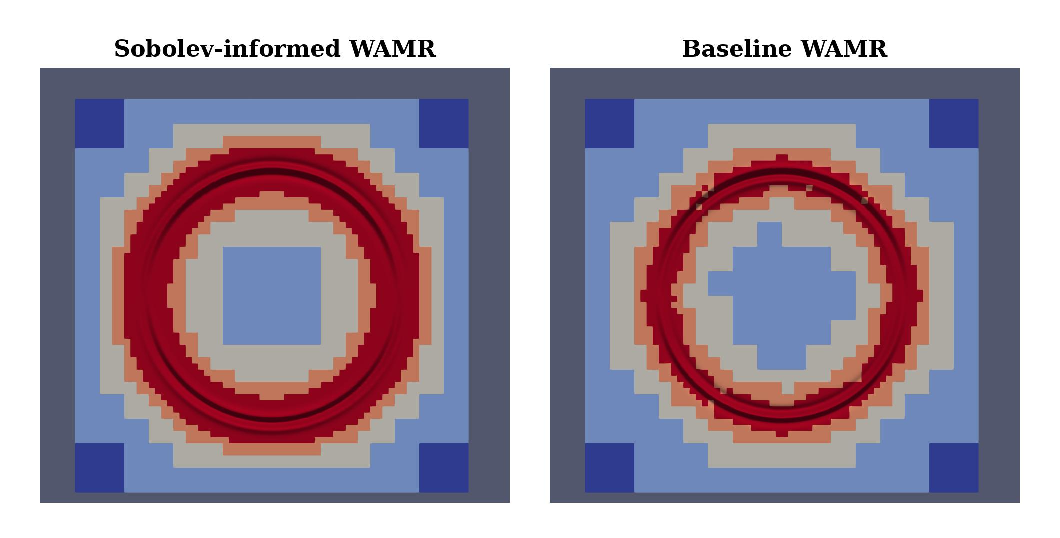
\includegraphics[width=0.85\textwidth]{Figures/Appendix/sobolev_wamr_labeled_side_by_side.pdf}
\caption{
Representative comparison of the adaptive mesh generated by the baseline wavelet AMR criterion and the Sobolev informed AMR criterion. The red areas represent areas of higher refinment the blue areas represent the areas with lower refinment. The Sobolev informed criterion includes derivative information in the refinement indicator, which changes where grid points are allocated. The oscillatory ring corresponds to the outward propagating dipole pulse. Notice that the sobolev inspired refinement produces a much more symmetric refinement. The Sobolev inspired criteria is more expensive but refines around the region of interest better.
}
\label{fig:sobolev amr mesh comparison}
\end{figure}

Figure~\ref{fig:sobolev amr constraints} shows the divergence constraints for the electric and vector potential fields. These quantities provide a direct measure of the constraint violation during the evolution. The comparison shows how the Sobolev informed refinement criterion affects the constraint preserving behavior of the evolution relative to the baseline wavelet criterion. Notice how much better the sobolev inspired does relative to the base case.

\begin{figure}[t]
\centering

\subfloat[$L_2$ norm of $\nabla_i E^i$.]{%
    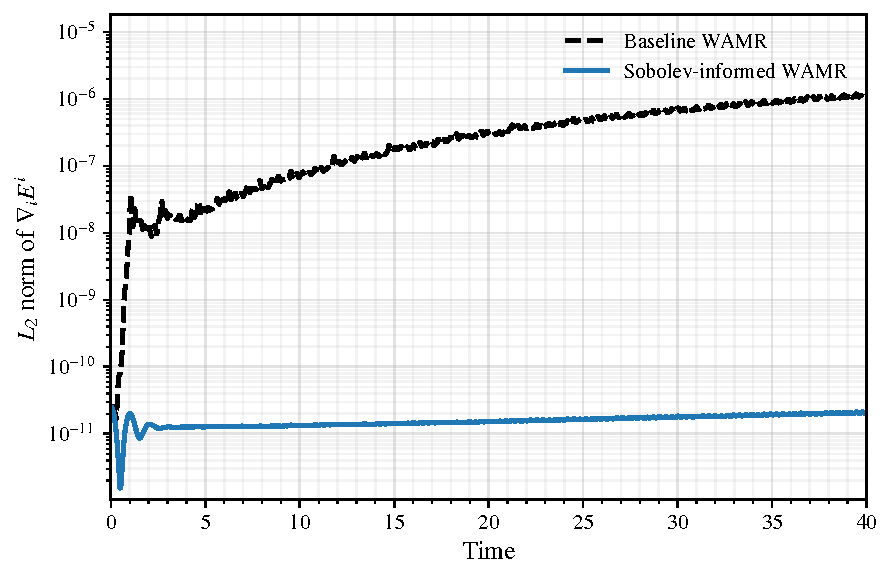
\includegraphics[width=0.48\textwidth]{Figures/Appendix/DivE_wavelet_tolerance_comparison.pdf}%
    \label{fig:sobolev amr dive}%
}
\hfill
\subfloat[$L_2$ norm of $\nabla_i A^i$.]{%
    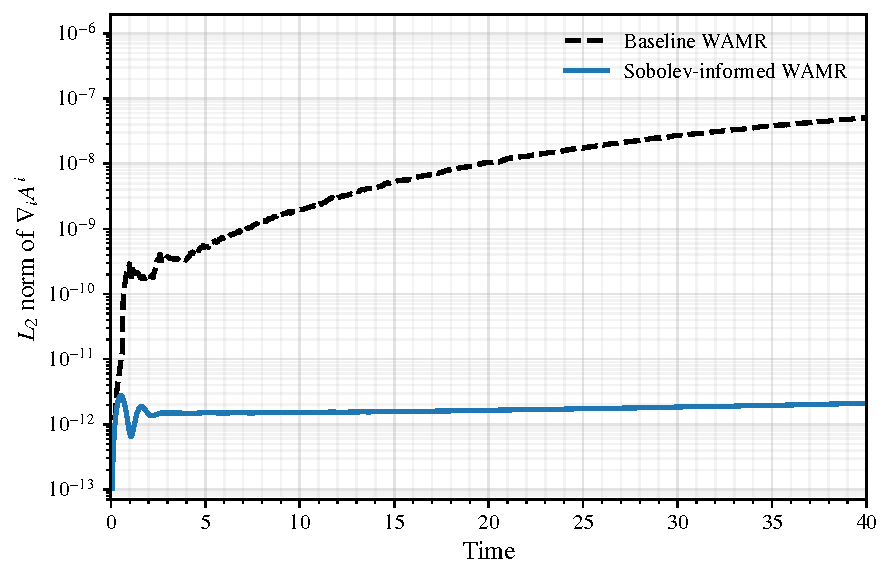
\includegraphics[width=0.48\textwidth]{Figures/Appendix/DivA_wavelet_tolerance_comparison.pdf}%
    \label{fig:sobolev amr diva}%
}

\caption{
Constraints for the baseline wavelet AMR and Sobolev informed AMR refinement criteria. The left panel shows the $L_2$ norm of the electric field divergence constraint, while the right panel shows the corresponding divergence for the vector potential. These quantities are used to assess whether the modified refinement indicator improves or degrades the constraint behavior of the evolution.
}
\label{fig:sobolev amr constraints}
\end{figure}

Figure~\ref{fig:sobolev amr efficiency} compares the number of active mesh points and a measure of the grid efficiency. The number of active mesh points, $N_{\mathrm{mesh}}$, measures the size of the adaptive grid and is therefore a proxy for the computational cost of the evolution. A refinement strategy that achieves comparable or smaller constraint violations using fewer mesh points is more efficient.

To quantify this tradeoff, we define the grid efficency as:
\begin{equation}
    \eta
    =
    \frac{1}{C_{\mathrm{tot}} N_{\mathrm{mesh}}^2},
    \label{eq:sobolev amr grid efficiency}
\end{equation}
where $C_{\mathrm{tot}}$ is the total constraint measure and $N_{\mathrm{mesh}}$ is the number of active mesh points. In this work, the total constraint measure is constructed from the divergence constraints as
\begin{equation}
    C_{\mathrm{tot}}
    =
    C_{\nabla E}
    +
    C_{\nabla A},
    \label{eq:sobolev amr total constraint}
\end{equation}
where $C_{\nabla E}$ and $C_{\nabla A}$ denote the $L_2$ norms of the corresponding divergences. With this definition, larger values of $\eta$ indicate that a simulation achieves smaller constraint violation for a given mesh size. The factor of $N_{\mathrm{mesh}}^2$ penalizes simulations that reduce the constraint violation only by using substantially more grid points.

\begin{figure}[t]
\centering

\subfloat[Number of active mesh points.]{%
    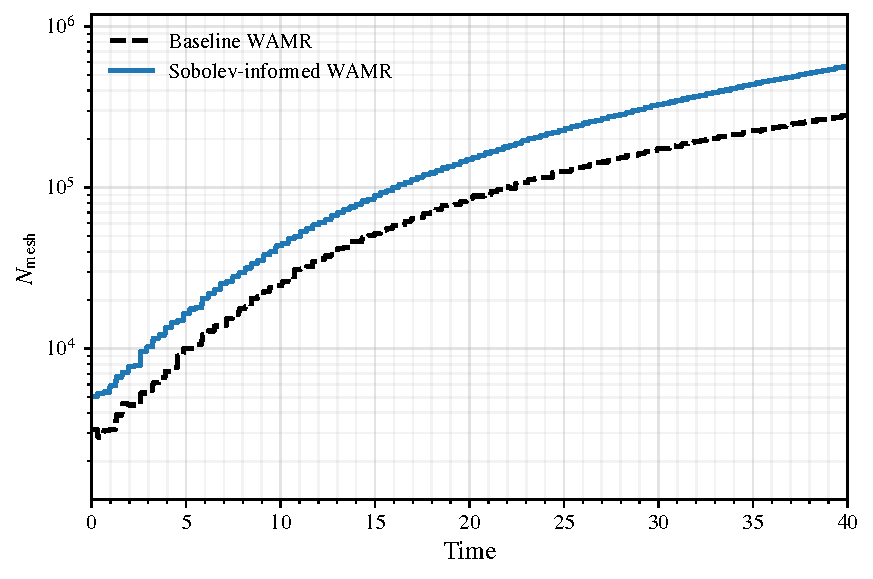
\includegraphics[width=0.48\textwidth]{Figures/Appendix/mesh_size_wavelet_tolerance_comparison.pdf}%
    \label{fig:sobolev amr mesh size}%
}
\hfill
\subfloat[Grid efficiency.]{%
    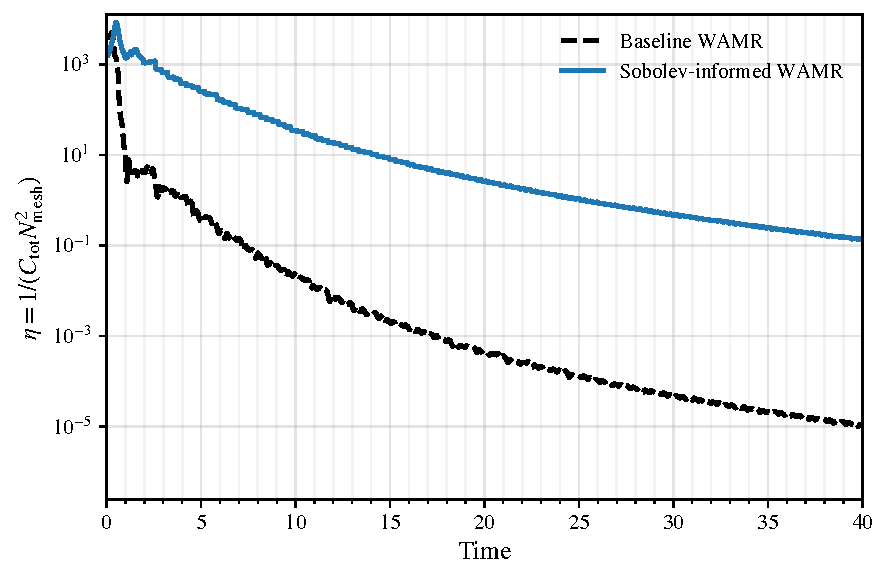
\includegraphics[width=0.48\textwidth]{Figures/Appendix/grid_efficiency_wavelet_tolerance_comparison.pdf}%
    \label{fig:sobolev amr grid efficiency}%
}

\caption{
Mesh size and grid efficiency for the baseline wavelet AMR and Sobolev informed AMR refinement criteria. The left panel shows the number of active mesh points $N_{\mathrm{mesh}}$, which serves as a proxy for computational cost. The right panel shows $\eta = 1/(C_{\mathrm{tot}}N_{\mathrm{mesh}}^2)$. Larger values of $\eta$ indicate smaller constraint violation for a given mesh size, and therefore a more efficient use of grid points.
}
\label{fig:sobolev amr efficiency}
\end{figure}